%% Hardware Metapaper Template for the Journal of Open Hardware, v.1

\documentclass[a4paper]{article}

\usepackage{lmodern}
\usepackage[T1]{fontenc}
\usepackage[utf8]{inputenc}
\usepackage{amssymb,amsmath}
\usepackage{todonotes}
\usepackage{caption, subcaption}

\usepackage{hyperref}
\hypersetup{unicode=true,
            pdfborder={0 0 0},
            breaklinks=true}
\urlstyle{same}

\usepackage{longtable,booktabs}
\IfFileExists{parskip.sty}{%
\usepackage{parskip}
}{% else
\setlength{\parindent}{0pt}
\setlength{\parskip}{6pt plus 2pt minus 1pt}
}
\setlength{\emergencystretch}{3em}  % prevent overfull lines
\providecommand{\tightlist}{%
  \setlength{\itemsep}{0pt}\setlength{\parskip}{0pt}}
\setcounter{secnumdepth}{0}

%% \date{}


\title{OpenPodcar: an Open Source Vehicle for Self-Driving Car Research}
\usepackage{authblk} 
\author[1,2]{Fanta Camara}
\author[2]{Chris Waltham} 
\author[2]{David Churchill}
\author[1,2]{Charles Fox} 
\affil[1]{Institute for Transport Studies, University of Leeds, UK} 
\affil[2]{School of Computer Science, University of Lincoln, UK}
\renewcommand\Affilfont{\itshape\small}

\begin{document}
\maketitle


% Include your abstract here MAX 250 words
\begin{abstract}
Autonomous vehicles, also known as 'Self-Driving Cars', is a fast-moving research field with big investments from both academia and the industry. Open source software for localisation, mapping and control is widely available but hardware components are often protected, making it difficult for researchers with low resources to test their new algorithms on realistic vehicle platforms. Here, we thus introduce OpenPodcar, an open source hardware platform based on a off the shelf, hard canopy, mobility scooter that uses Ackerman steering. We make available both hardware and software designs used to convert the mobility scooter into a low-cost and fully autonomous platform. The open source platform consists of (a) hardware components: CAD designs, bill of materials, and build instructions; (b) Arduino, ROS and Gazebo control and simulation software files which provide standard ROS interfaces and simulation of the vehicle; and (c) higher-level ROS implementations of standard robot control, including the move\_base interface with TEB (Timed-Elastic-Band) planner which enacts command to get the vehicle move from one pose to another. The platform is large enough to transport one person at speeds up to 15kmh, for example for use as a last-mile autonomous taxi service or to transport delivery containers similarly around a city center. It is also small and safe enough to be parked in a standard research lab and be used for realistic human-vehicle interaction studies. Together with its low costs, around USD7,000 in total in 2022, OpenPodcar thus forms an ideal balance between real world utility, safety, cost and research convenience platform.
\end{abstract}

\begin{longtable}[]{@{}l@{}}
\begin{minipage}[t]{0.97\columnwidth}\raggedright\strut


%% Hardware Metapapers are structured summaries of open hardware projects. Word limit: 4,500 words

\subsection{Metadata Overview}\label{h.akaipbqoqfs8}

Main design files: \url{https://github.com/OpenPodcar}

Target group: researchers and hobbyists interested in autonomous vehicle research and robotics. 

Skills required: Mechanical assembly – easy; electrical assembly – intermediate; Software – advanced.

Replication: The work in this project is being replicated on a courrier-type manually-driven platform for a vehicle manufacturer. The current OpenPodcar is being used by some of the authors for human-robot interaction experiments and a similar mobility scooter will be built based on the documentation to improve its accuracy.



\subsection{Keywords}\label{h.kdz351yp7g7c}

{Autonomous Vehicles, Open Source Hardware and Software.}

\strut\end{minipage}\tabularnewline
\bottomrule
\end{longtable}


\subsection{Introduction}\label{h.pnj38xyr5dyy}

The use of open source hardware (OSH) allows for more effective and accessible sharing and collaboration among researchers \cite{fisher2012open}, as well as more accessible entry-level projects such as examples from Oxer and Blummings (2009)\todo{who?}. OSH brings a number of benefits to a research community, as a common context for results and accessible platform with which to test new ideas allows for more engagement, leading to a more mature field of study. Specific requirements for such a platform are that it needs to be as low cost as possible, and easy to build. This is to enable the community to reproduce and use it. Consumer levels of safety and reliability are not required, preferring to minimise cost, though research standards of safety and reliability are required.

Open source simulation platforms are widely available for autonomous vehicle research, such as CARLA \cite{dosovitskiy2017carla}, SUMMIT \cite{cai2020summit}, FLOW\footnote{https://flow-project.github.io/}, DEEPDRIVE\footnote{https://github.com/deepdrive/deepdrive}, AirSim\cite{shah2017airsim}, LGSVL Simulator \cite{rong2020lgsvl} and Gym-Duckietown \cite{chevalier-boisvert2018duckietown}. In contrast, it is currently almost impossible to build any large hardware design that does not incorporate non-open designs or make use of non-open designs as tools during construction. The present OpenPodcar is thus currently only "weak" OSH, like the Arduino, because it depends on the use of a patented donor vehicle and uses sensors or other components e.g. 3D Lidar that are also patented. It is intended as a basis for future work which could replace the patented components with open interfaces to progress it to "deeper" OSH.


Main objectives with this platform: portability,  accessibility, adaptability, affordability.

\subsubsection{Donor vehicle base}    
A Pihsiang TE-889XLSN hard-canopy scooter (branded in UK as Shoprider Traverso, \cite{shoprider2006}) is used as the podcar platform. It is an electric mobility scooter powered by two 12V batteries connected in series to provide 24V operating voltage and containing 75Ah. In its standard configuration, the donor vehicle’s steering is controlled by a human operated loop handle bar. The speed and braking systems are both powered by an electric motor and an electric brake via the trans-axle assembly, controlled by an AC2 digital controller receiving different voltage signals to drive forward or brake. The manual speeding and braking systems are controlled by three buttons connected in series on the handle bar. A toggle switch in parallel with a resistor (10k$\Omega$) to choose speed mode high or low; A speed dial knob via a variable resistor (20k$\Omega$) to choose a maximum speed value; A throttle lever connected with a potentiometer (5k$\Omega$), 2.5k$\Omega$ to 2.6k$\Omega$ for each side to speed or brake. 

\subsubsection{Open source software base}

ROS, is `an open source operating system' for robots based on a publish-subscribe pattern \cite{quigley2009ros}, which is the robotics community’s standard interface. Building on top of ROS, the `ROS ecosystem’ is a loosely-defined collection of open-source ROS packages with variously accepted standard message formats which act as conventional interfaces to enable many community packages to work together and to act as swappable alternatives for one another. ROS drivers are packages in the ecosystem which wrap robot hardware with standard ROS interfaces. ROS launch files are stored configurations of ROS nodes that can be run using one command from a terminal. These are used widely by ROS packages to quickly launch the nodes required for a certain task at the same time.

Gazebo \cite{koenig2004design} is a robotics 3D physical simulation and 3D graphics display tool, separate from, but designed to integrate with ROS, and which is the robotics community standard simulator. An example of one such project that makes use of Gazebo in conjunction with ROS is reported by Qian et al 2014) which presents an example of a project in which the hardware and software are developed in parallel, making use of ROS (for providing the software interface) and Gazebo (for testing hardware that doesn’t yet exist in the real world). 


\subsubsection{Related systems}

SMART [CITE] is a design to modify an existing donor golf cart vehicle for automation research, developed by MIT and Singapore. The vehicle is a similar size and power to OpenPodcar but is not open source. Beetlebot \cite{beetlebot} is a OSH system similar to OpenPodcar but for last-mile freight delivery, without human carrying capacity, and including ROS integration. Open Source Ecology (OSE) [CITE??] is an ambition project which ultimately aims to develop Deep OSH vehicles including a car and tractor, via a process of progressively deeper Shallow OSH designs.  OSE is optimised for reliability and for users in developing countries so uses hydraulic power rather than electric as used in OpenPodcar. Several functioning OSH designs for large cars exist, including Apollo\footnote{https://github.com/ApolloAuto/apollo}, PixBot\footnote{https://gitlab.com/pixmoving/pixbot} and OSVehicle Tabby \footnote{www.openmotors.co/tabbyevo/}. AutoRally\footnote{https://autorally.github.io/} \cite{goldfain2019autorally} developed by researchers at Georgia Tech and the Berkeley Autonomous Race Car (BARC\footnote{www.barc-project.com/}) are small-scaled autonomous vehicles for research, but only BARC includes ROS integration. Autoware \cite{kato2018autoware} is a heavyweight open source software project to construct a ROS based automation stack for large on-road cars with power on-board computers. The state of Georgia, in the USA, provides a level 3 open-source autonomous vehicle based on a Ford-Edge at the Curiosity Lab at Peachtree Corners \footnote{https://www.peachtreecornersga.gov/businesses/curiosity-lab-at-peachtree-corners}, where technologists and researchers can use the platform in the smart city environment free of charge. 

%https://ieeexplore.ieee.org/document/8926794


%https://ieeexplore.ieee.org/document/8813784



\section{(1) Overall Implementation and design}\label{h.1u7vph94gfbt}

\subsection{Mechanical Modification for Steering}

To automate steering, a Gimson GLA750-P 12V DC linear actuator with position feedback is mounted between an anchor on the underside of the chassis and the car's front axle via bearings.  This actuator has a 8mm/s full load (750N) speed and 250mm stroke length (installation length is 390mm).  

To access the underside of the vehicle, two axle stands were used as shown in Fig. \ref{fig:axelStands}. There is an existing hole in the right front wheel axle. The linear actuator was mounted via a rear hole to the left side of the front chassis and connected through the front hole of the actuator with the hole in the car's right front wheel axle via bearings as shown in Figs. \ref{fig:actuatorMounted} and \ref{fig:steering}.


\begin{figure}
	\centering
	\begin{subfigure}{0.45\textwidth}
		\centering
		\includegraphics[scale=0.29]{hardware/onAxles.jpg}
		\caption{Tilting the vehicle using two axle stands, to enable access to the underside. (Note also lidar mounted to roof.)}
		\label{fig:axelStands}
	\end{subfigure}	
	\quad
	\begin{subfigure}{0.45\textwidth}
		\centering
		\includegraphics[scale=0.23]{hardware/steeringActuatorMounted.jpg}
		\caption{Underside with linear actuator added for steering.}
		\label{fig:actuatorMounted}
	\end{subfigure}
	\caption{Vehicle mechanical modification}
\end{figure}


\begin{figure}[h]
	\includegraphics[width=\columnwidth]{hardware/steering1.png}
	\caption{The bottom view of front wheels steering relationship including geometric coefficients}
	\label{fig:steering}
\end{figure}


\subsection{Electronics and Firmware}

\begin{figure*}[h]
	\includegraphics[width=\linewidth]{hardware/circuitDiagram.png}
	\caption{Circuit diagram for electronic modifications.}
	\label{fig:circuitDiagram}
\end{figure*}


The new vehicle electronics, that require different voltage power supplies (cf. Fig. \ref{fig:circuitDiagram}), were originally arranged on an acrylic board mounted under the seat of the vehicle, as shown in Fig. \ref{fig:initial_electronics}. With this initial electronic setup, we were able to drive the vehicle with a remote control but over time we experienced a lot of disruptions with small wires not always holding in place on the acrylic board because in most cases tape was used to hold them together. After a year without using the vehicle due to covid-19, when we returned to the lab, the podcar battery started not working properly and it became almost impossible to drive the vehicle for more than 5min without also having wires disconnecting.

To solve this issue and robustify the electronics modifications, we thus designed and manufactured a PCB (Printed Circuit Board), as shown in Fig.~\ref{fig:pcb_assembled}. A PCB is more convenient, because it reduces the number of small wires between the components by having them directly drawn on the board. The PCB is composed of two DC-DC Buck converters with an XL4016 regulator, an Arduino Uno, an MCP4725 DAC (Digital-Analog Converter), a Pololu JRK 21v3 motor controller with position feedback for the linear actuator, 2 resistors (10k$\Omega$ and 100k$\Omega$) for the potential divider. We 3D printed parts to support the mounting of the LCD and the 3D LIDAR to the board. A 3D printed enclosure was designed to protect the PCB board, as shown in Fig.~\ref{fig:pcb_enclosure}.

\begin{figure}
	\centering
	\includegraphics[width=0.5\columnwidth]{hardware/pic_boards.jpg}
	\caption{Initial electronics on acrylic board.}
	\label{fig:initial_electronics}
\end{figure}

\begin{figure}
	\centering
	\begin{subfigure}{0.45\textwidth}
		\centering
		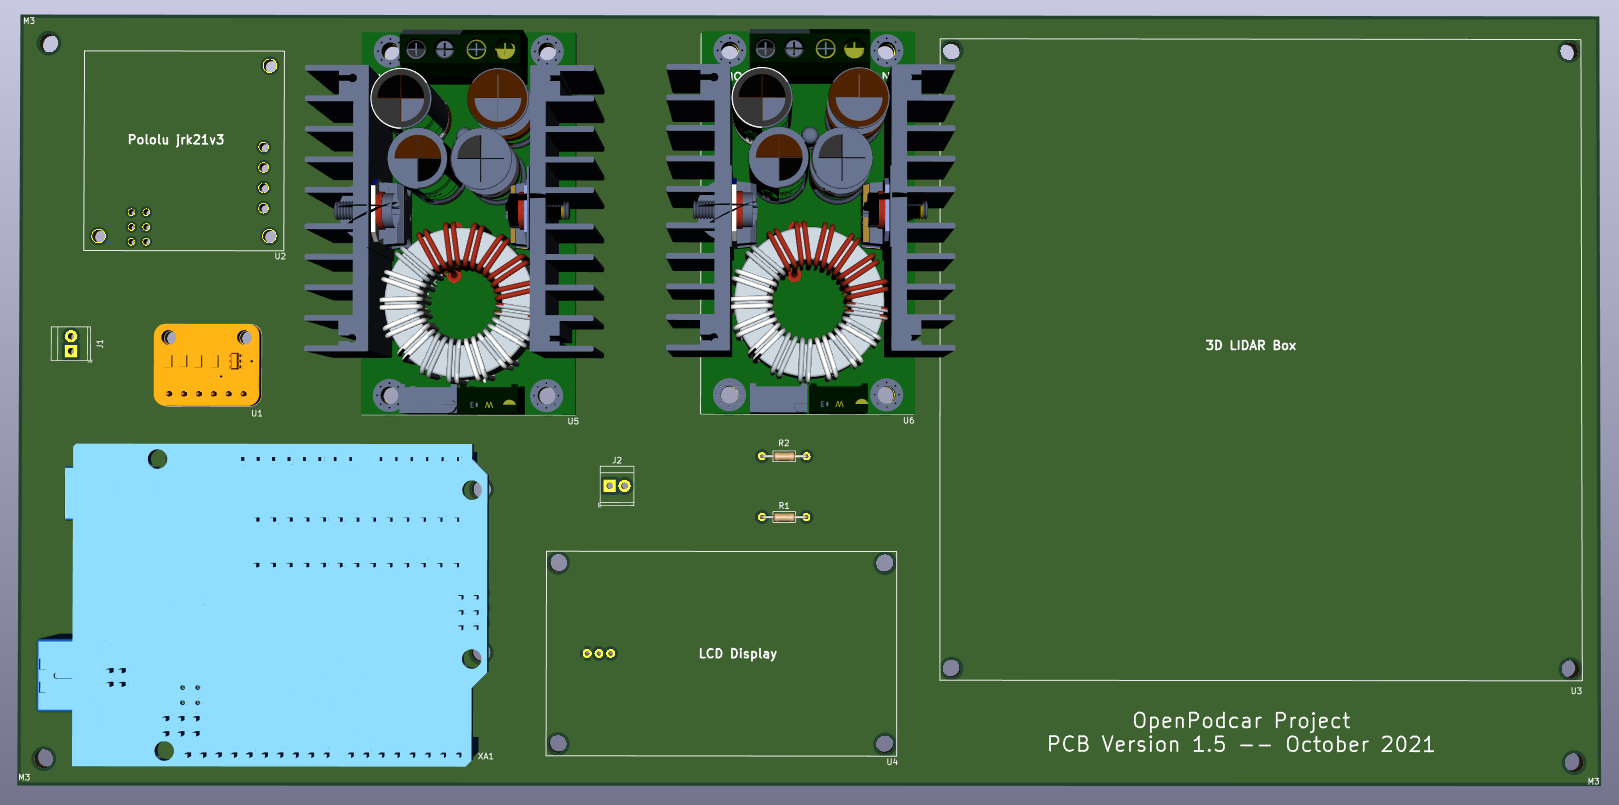
\includegraphics[width=\columnwidth]{hardware/pcb_version_1_5_pic1.png}
		\caption{PCB Design.}
		\label{fig:pcb_design}		
	\end{subfigure}
	\quad
	\begin{subfigure}{0.45\textwidth}
		\centering
			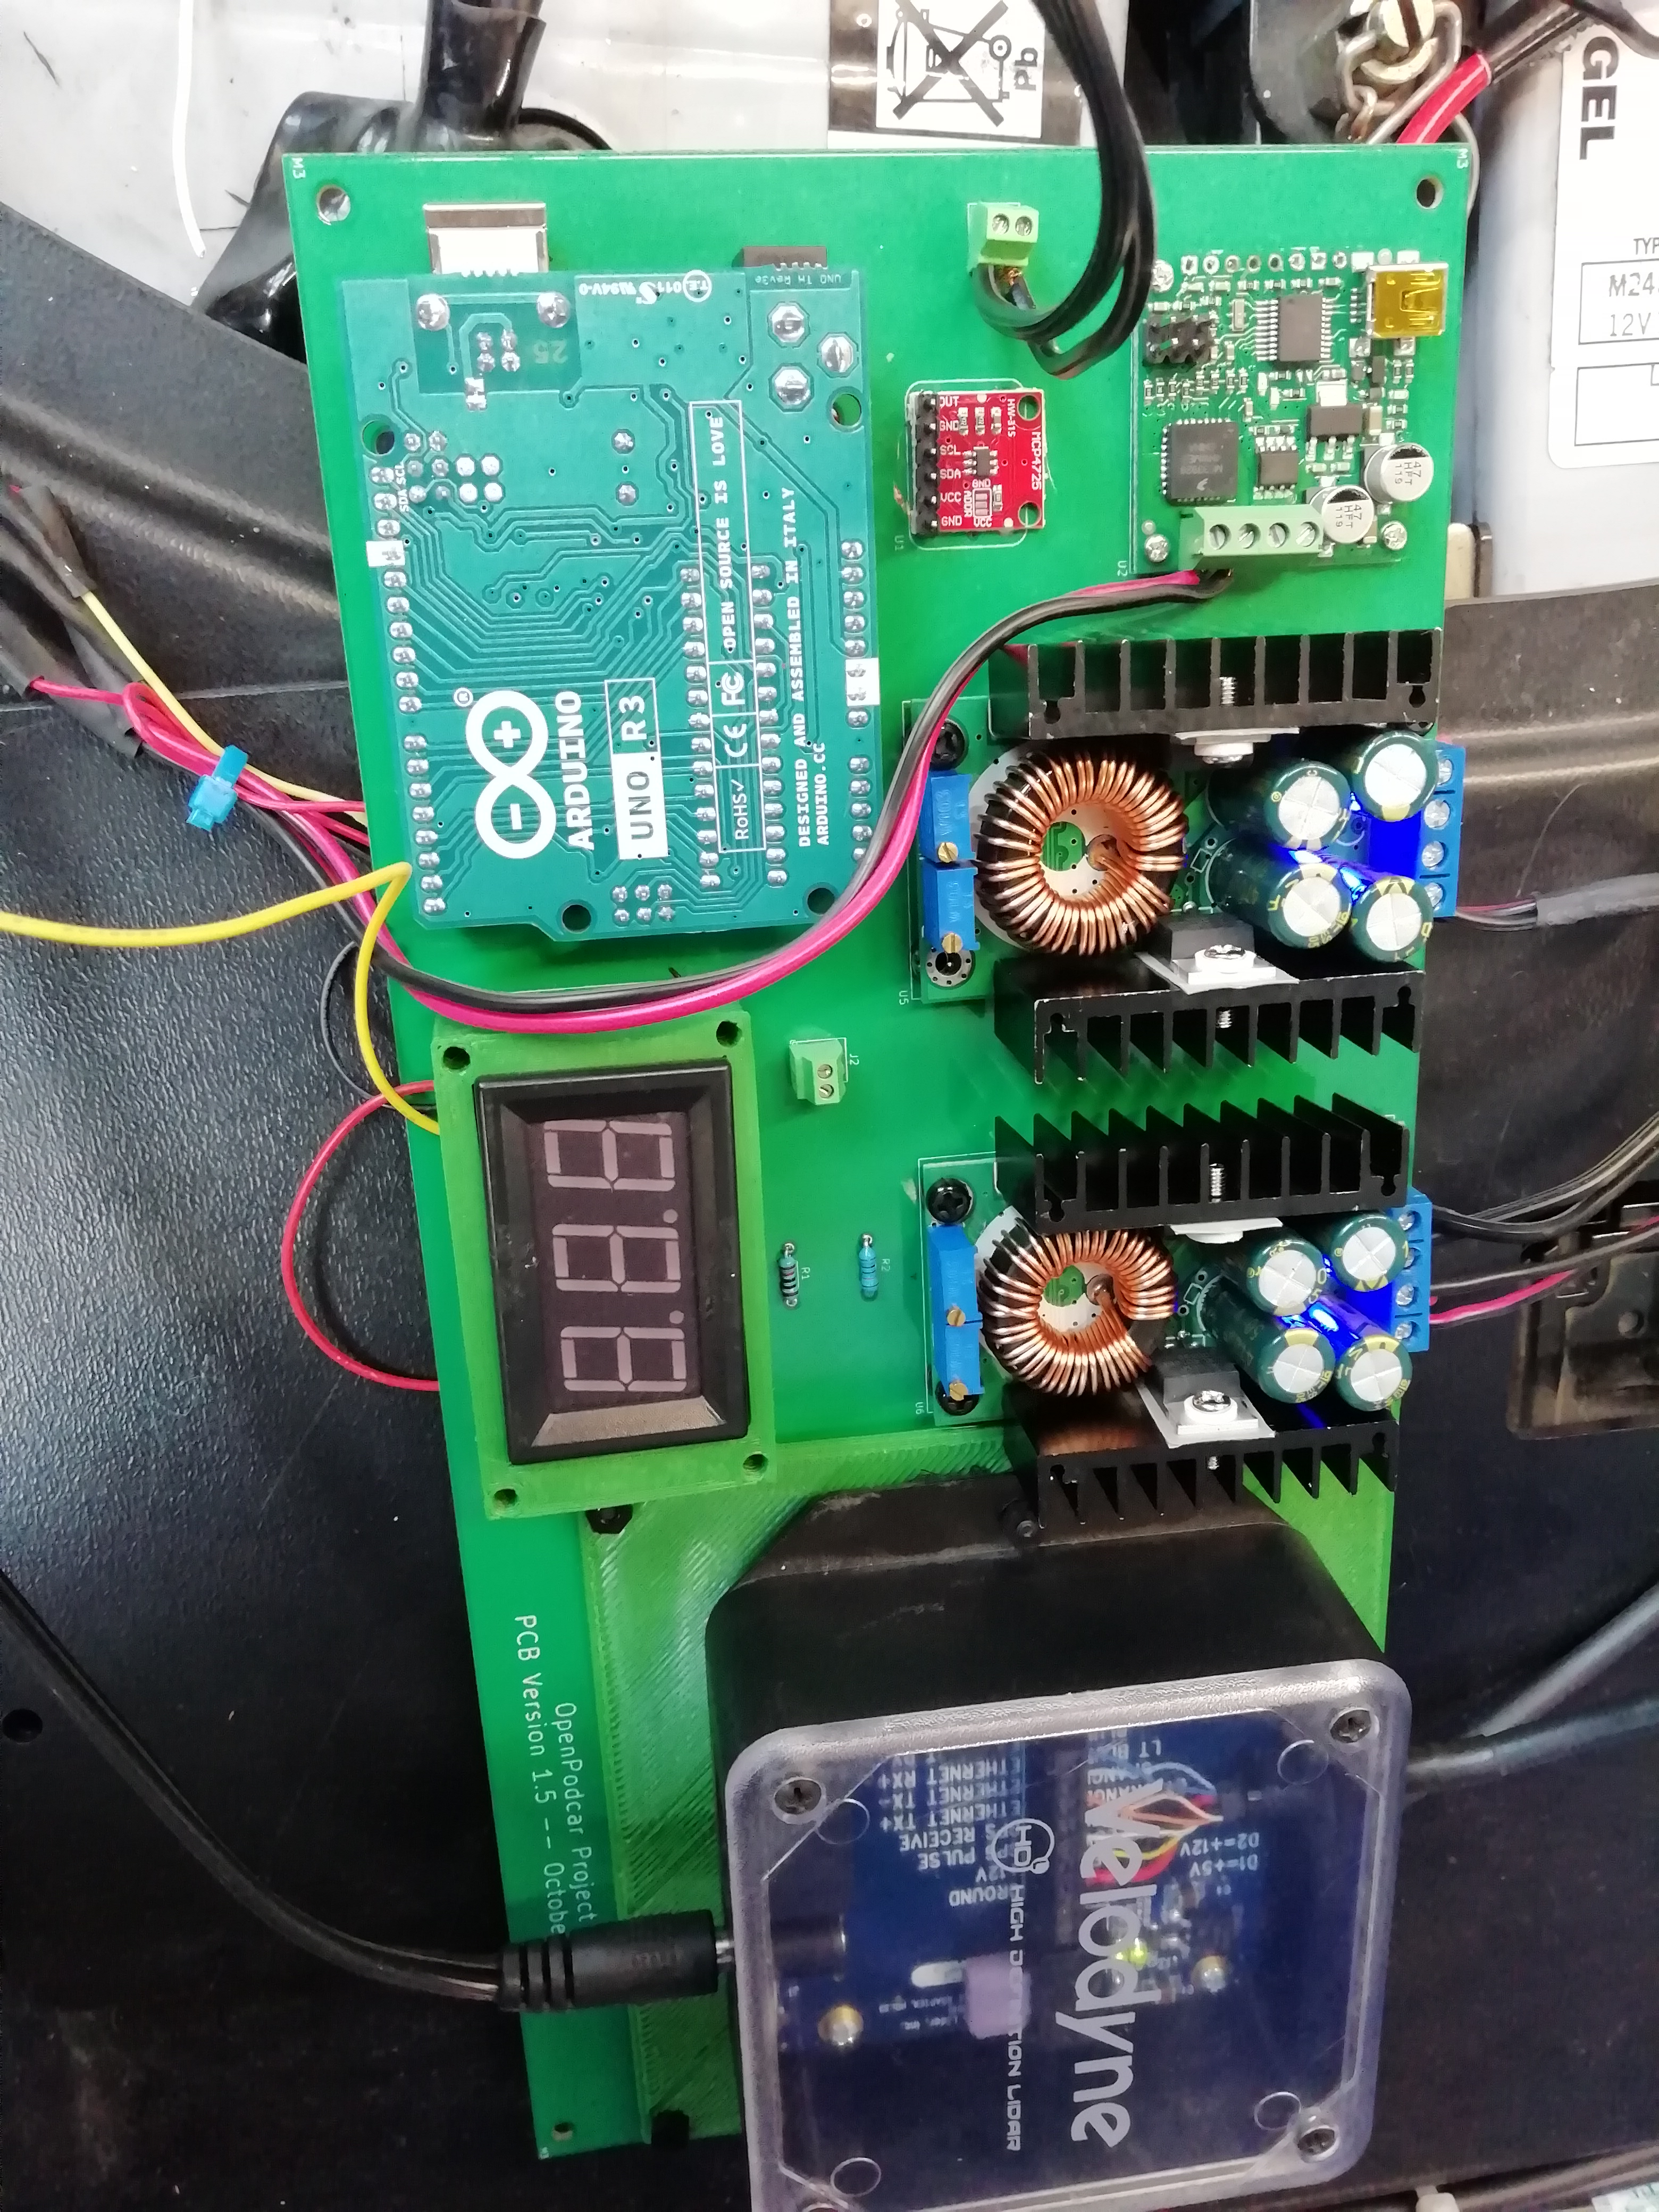
\includegraphics[width=0.5\columnwidth, angle=90]{hardware/pcb_podcar.jpg}
			\caption{PCB assembled and currently used.}
			\label{fig:pcb_assembled}
	\end{subfigure}	
	\caption{Initial electronics and PCB boards}
\end{figure}


\begin{figure}
	\centering
	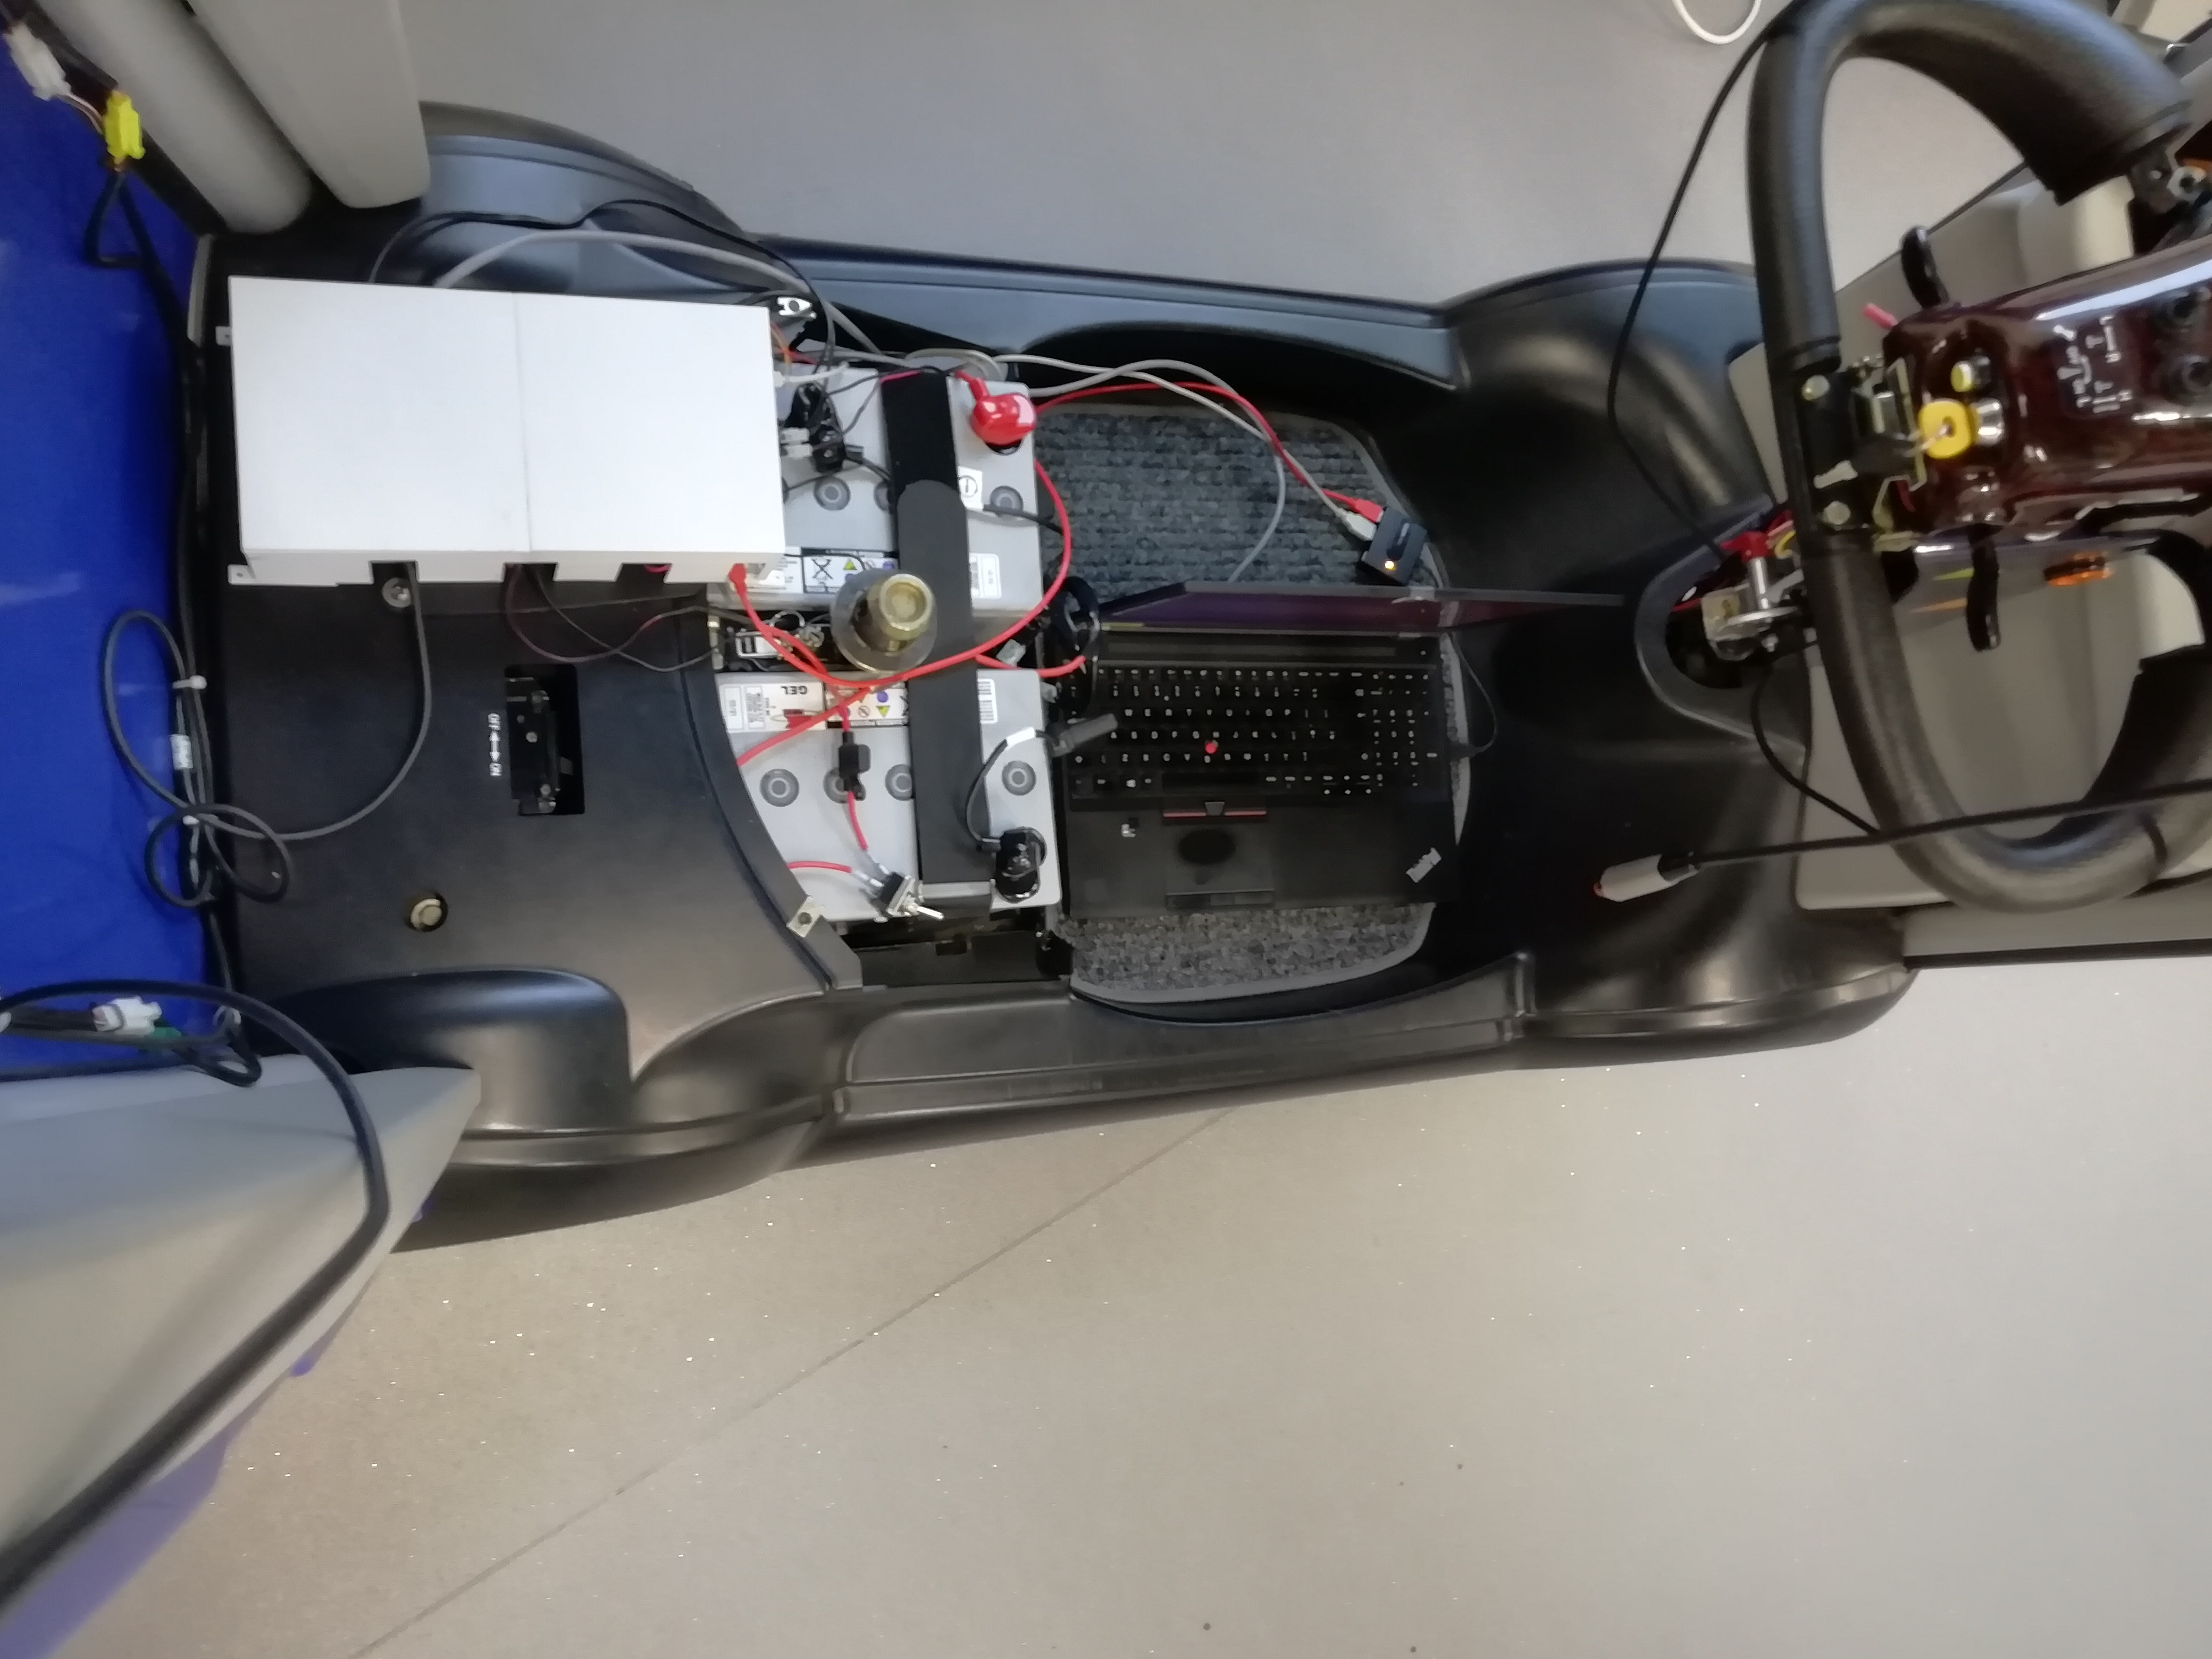
\includegraphics[width=0.7\columnwidth]{hardware/pcb_enclosure.jpg}
	\caption{View of the vehicle interior with the PCB enclosure and laptop.}
	\label{fig:pcb_enclosure}
\end{figure}



\subsubsection{Steering control system}

The front wheels are steered by a Pololu jrk21v3 PID controller, and it takes serial port desired positions as input. It also takes feedback position information as an analog voltage from the linear actuator as an input. It outputs analog high-power voltages to the linear actuator. A Windows app is required (once) to set the PID parameters for the linear actuator, the detail of this processs is explained in the documentation. 

The relationship between the required central turning angle $\theta$ of the pair of front wheels and extending length $l$ of linear actuator is,    
\begin{gather}
\theta = \alpha - \arctan(\frac{W}{2H}) \\
% update W and H in figure. W is the width between two front wheels and H is the distance between front wheel and rear wheel.
\beta = \alpha -\frac{\pi}{2}\\
x = r_1 * \cos(\beta) \\
y = r_1 * \sin(\beta) \\
l = \sqrt{(x_0-x)^2 + (y_0-y)^2} - L + l_0    
\end{gather}    
Where $r_1$, $x_0$, $y_0$, $W$, $H$ and $L$ are the geometric coefficients shown in Fig.1. Among them, the value of $y_0$ is negative. $l_0$ is the initial value of the linear actuator position feedback.

% related to:
%'889XLSBN CAN Traveso Spare Parts List' page 29, 30, 32, 33, 34, 37, 38, 40 and 41;
%'Shoprider Scooter Service Manual Live Document' page 7, 8, 14 and 16.  

Table \ref{tab:linear_actuator} shows the acceptable commands for the linear actuator, giving commands outside this range may mechanically destroy the system.  
\begin{table}
	\begin{center}
	\caption{Linear actuator acceptable command ranges.}
	\label{tab:linear_actuator}
		\begin{tabular}{ c c }
			\hline
			FA:cmd     &  Effect \\
			2500    &    max right i.e $\sim$ -45 deg \\
			1900    &    center i.e $\sim$ 0 deg \\ 
			1000    &    max left i.e $\sim$ +45 deg \\
			\hline\\
		\end{tabular}
	\end{center}   
\end{table}
 



\subsubsection{Speed controller system}

An Arduino UNO \cite{oxer2011practical} is used to send electric signals to the vehicle's motor controller in place of the donor vehicle’s paddle controller’s potentiometer. An Adafruit MCP4725 DAC is connected to the Arduino as in Fig. \ref{fig:circuitDiagram}, and used to send clean analog speed command voltages to the donor vehicle’s internal controller.

Arduino code is supplied in the distribution (/Arduino/ThrottleControlSerial.ino). When uploaded to the Arduino (using the standard Arduino IDE running on the laptop), it provides a simple serial port API running at 112000baud. It receives commands of the form “FA:210” as speed commands. Table \ref{tab:speed_commands} summarizes the range of speed commands and their corresponding output voltages. 

\begin{table}
\begin{center}
	\caption{Speed commands and their corresponding output voltages.}
	\label{tab:speed_commands}
	\begin{tabular}{ l c c }
		\hline
		Command   &    Voltage            &  Effect \\
		FA:0      &    0                  & stupid fast reverse  \\
		FA:80     &    $\sim 0.9$         & v fast reverse (ros limit) \\
		FA:132    &   $\sim 1.5$          & slowest reverse motion  \\
		&                       & dead zone - allows ignition \\
		FA:170    &    1.9                & stop - zero/home position \\
		FA:201    &    $\sim 2.3$         & slowest forward motion \\
		FA:240    &    $\sim 2.7$         & v fast forward (ros limit) \\
		FA:255    &    $\sim 3.0$         & stupid fast forward \\
		\hline\\
	\end{tabular}
\end{center}    
\end{table}

To start the ignition, the car safety system requires the control voltage to be in the dead range. A problem is that this doesn’t correspond precisely to any fixed speed bytes, due to the USB power issues.  But if we pick a number solidly in the center of the dead zone, such as 164, this will work for most USB supplies. (i.e. when the vehicle’s battery is flatter, the voltages provided to USB power by it are lower. For example, we might send 164 and get 1.9V instead of the usual 2.26V.) This may result in the vehicle not starting -- maybe by design or accident -- this produces a beep as is outside the start zone. 

The Arduino gets lower power e.g. max 4.9V instead of 5V, which gets divided by the DAC value. To deal with these instabilities, we added a potential divider at the battery to check the voltage and control the podcar accordingly, as in Fig. \ref{fig:potential_divider}. We provide a “BV” command in the Arduino serial protocol which allows callers to request the current battery voltage. This can then be used by the higher level (Python) systems to decide what speed bytes to sent, including compensating for the floating dead zone.

\begin{figure}
	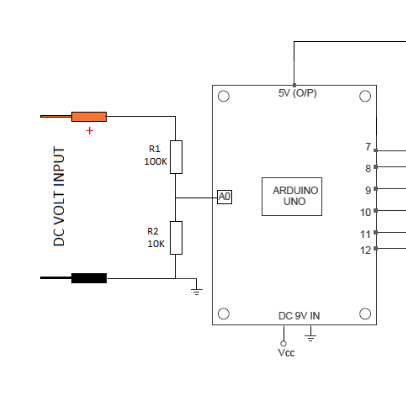
\includegraphics[width=0.5\columnwidth]{hardware/potential_divider.png}
	\caption{Potential divider linked to the battery}
	\label{fig:potential_divider}
\end{figure}


\subsection{3D Lidar Sensor}
A Velodyne VLP-16 lidar sensor is mounted on the vehicle roof using a small optical tripod (TODO give model). Note that optical devices have unusual physical mounting standards which use Imperial rather than metrics units.  This system is used by optics research based on optical table sizing. The lidar screws onto the tripod. The tripod is cabled-tied to the vehicle roof via  drilled holes at locations in Fig. TODO.  It is mounted at a 10 degree tilt downwards (to allow pedestrians to be most clearly seen in the 16 scan lines).

\subsection{Physical vehicle software interface (ROS)}

A ROS interface to and from the physical vehicle is provided as illustrated in Fig.\ref{fig:meshSim} and described below. This was originally running on a Panasonic CF-19 Toughbook computer mounted on-board the vehicle (and powered from a DCDC converter from the  vehicle battery) running Xubuntu 16.04 (Xenial) and ROS Kinetic. But the tests showing the autonomous driving capabilities were done using a Lenovo ThinkPad P51 laptop for faster computation.

\begin{figure*}[h]
	\includegraphics[width=\textwidth]{software/rosnodes.png}
	\caption{ROS nodes and messages for low-level control.}
	\label{fig:meshSim}
\end{figure*}

\subsubsection{Control system interface}
The system expects to hear two incoming ROS control messages: speedcmd\_meterssec and wheelAngleCmd, which contain single floats representing the desired speed in meters per second, and the desired front wheel orientation in radians respectively.

These two messages are received by ROS nodes speedm2arduino and wheelAngle2Pololu, which are ROS drivers for the Arduino speed controller and the Polulo steering controller respectively.

\subsubsection{Manual joystick control}
Converters from a standard ROS USB joystick driver node to the speed and angle command interface messages are provided, by joystick2speedms and joystick2wheelAngle.  These use the $y$ axis of a joystick for speed and $x$ for steering.

\begin{figure}
	\centering
	\includegraphics[width=0.5\columnwidth]{hardware/testDrive.png}
	\caption{OpenPodcar test drive with remote control.}
	\label{fig:testDrive}
\end{figure}

\subsubsection{Lidar option}
Velodyne works with the velodyne ROS package. But it needs to be set up so we can talk to the Velodyne over Ethernet. The laptop must be on a wired network, not wifi. The IPs must be configured as in the velodyne, the steps are detailed in the build instructions. The default lidar IP is 192.168.1.201. 


\subsection{Universality of the design}\label{h.q32f2nclh4e5}

One of the biggest advantages of OpenPodcar is that the mechanical, electronics and software components can be easily ported to other vehicles/platforms and only require small changes on the software side to adapt it and fix some parameters specific to the new vehicle requirements. Some of the authors are currently porting the hardware and software stack to another type of vehicle. Cheaper sensors such as depth cameras or stereo cameras could be used instead of the 3D lidar. 



\section{(2) Quality control}\label{h.f8237gmzmwc6}

\subsection{Safety}\label{h.v60aduckfisj}

\subsubsection{Electronics Safety}

As shown in Fig.~\ref{fig:circuitDiagram}, a fuse is connected between the 24 battery of the vehicle and the system switch connected to the DC-DC converters on the PCB.   

The PCB board was heavily tested before and after assembling its components to ensure that once it is integrated into the vehicle, there would be any big issue. For instance, in Fig. \ref{fig:pcb_testing}, we used an external power supply and a multimeter to measure the voltage across the PCB components, check the safety of the board and ensure that the components work as expected.  


\subsubsection{Steering Control System Safety}

Limitations were added in the steering controller for the linear actuator commands, to only allow the vehicle to accept and execute input values within the range that will keep the mechanical mounting safe.


\subsubsection{Speed Control System Safety}

Autonomous vehicles can present a significant hazard to people and the environment in which they operated. Damage to surroundings and possible injury to operators and bystanders could result from inappropriate use or malfunction. It is essential that a suitable emergency stop system is implemented in all autonomous vehicles. Given the development platform nature of the OpenPodcar, a safety mechanism which stops the vehicle under fault conditions is an especially important part of the design. The design thus requires a series of positive heartbeat signals to be present and timely and also a dead-mans handle (DMH) to be depressed by a human experimenter at all times, in order for a hardware relay to actively continue to supply power from the vehicle’s batteries to all other systems. The relay will naturally cut out if these signals are absent for any reason, including failures in the safety systems themselves.

Implementing and testing this safety system should be undertaken with the drive wheels of the vehicle raised off of the ground, allowing for checks to be made of the DMH without the risk of the vehicle speeding off out of control.

The speed controller on this particular mobility scooter has a dead zone at around 2.5V on its speed input signal which corresponds to drive wheels stopped. Above the dead zone and up to 5V being forward control values and 0V to below the dead zone being reverse control voltages.

These values were checked using a multi-meter prior to implementing the Arduino controller and DAC.  This means that if the DAC output from the Arduino where to fail and 0V for example is applied to the mobility scooters speed controller input, the vehicle would respond by spinning the drive wheels backwards at full throttle. This being a dangerous eventuality, it is very important in terms of safety to ensure this situation can not arise.

A two stage approach is used to reduce this risk. Refer to the schematic diagram DMH section in conjunction with this description.

\paragraph{Stage 1 – Relay.} A relay is used which interrupts the mobility scooter’s key ignition circuit. If the relay is not energised by the presence of a 5V supply to the Arduino, the vehicle’s movement is disabled. This effectively ensures that if the Arduino is non-functional, for example its power supply has failed or it has been unplugged from the USB port of the control PC and there is a danger that the DAC is not producing the control systems required voltage, the scooter is automatically disabled by effectively switching it off.

\paragraph{Stage 2 – DMH Switch.} A sturdy push button is used which also interrupts the vehicle's key ignition circuit. If the Podcar operator detects any abnormality in operation during operation, he/she simply releases pressure from the DMH switch and the vehicle’s movement is disabled. The DMH switch is wired in series with the relay in the key ignition circuit ensuring that if both the relay contacts and the DMH switch are closed, this is the only condition where the Podcar movement is active.

The addition of the Relay and the DMH Switch are essential for safe operation, especially where new unproven autonomous control systems are in development.

A photograph of the installed system is shown in Fig. \ref{fig:relay}.

\begin{figure}
	\centering
	\begin{subfigure}{0.45\textwidth}
		\centering
		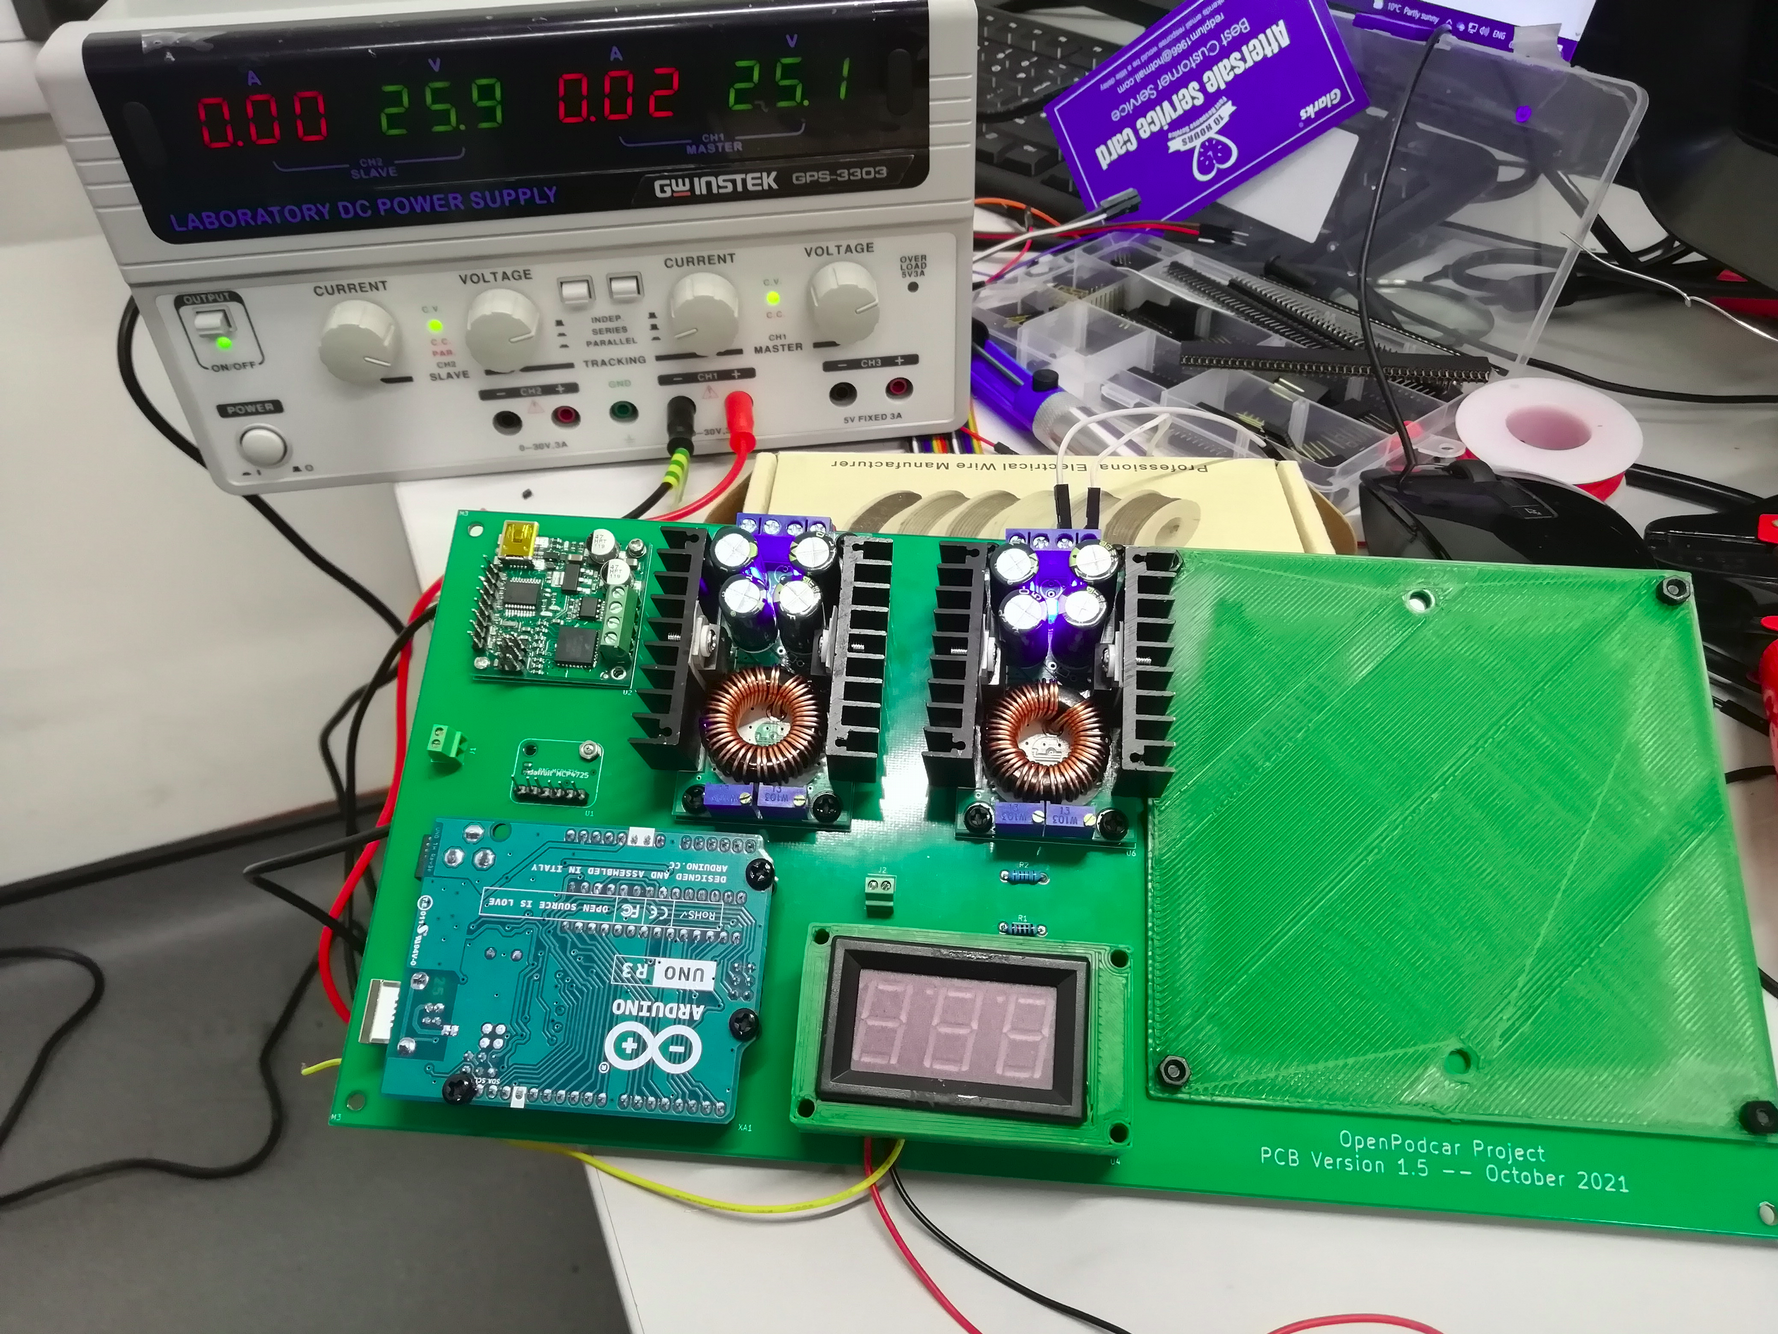
\includegraphics[width=0.75\columnwidth]{hardware/pcb_testing.png}
		\caption{Testing the PCB board.}
		\label{fig:pcb_testing}
	\end{subfigure}
	\quad
	\begin{subfigure}{0.45\textwidth}
		\centering
		\includegraphics[width=0.9\columnwidth]{hardware/pic_relay.jpg}
		\caption{Steering console showing newly added relay (with lit LED)}
		\label{fig:relay}
	\end{subfigure}
	\caption{Safety features for the vehicle}
	
\end{figure}


\subsection{General testing}\label{h.wbekh9ay82yu}

%In this section, details can be provided on the testing of hardware functionalities, that are not directly essential for precision operation of the hardware in the given context (which are in turn, where applicable, handled under Calibration), such as automated movements to position the hardware, repeatability of tool exchanges, recyclability, water-tightness, weight or other possibly relevant characteristics. We encourage the authors to characterise all appropriate functionalities of the hardware, if not already described elsewhere (add reference instead). The testing should define the safe/reliable limits in which the components can be operated (e.g. step size and repeatability of linear motion, force ranges, ratio of devices with leaks when built in a workshop, etc).This will enhance the usability of the hardware or method in other contexts. Again: Detailed instructions belong in documentation; here, provide a summary ~instead.

Summary of testing\\
The platform was developed between 2018 and 2022, it has thus been  extensively tested. In particular,  

Before testing the full automation capability of the software, we first tested that all the components worked well when the vehicle is controlled with a joystick.


\section{(3) Application}\label{h.f78bi3oom0mu}

\subsection{Use case(s)}\label{h.4q5g9edishy3}

%\subsubsection{Subsections}\label{h.qz4dez1pbkv1}

%We encourage the demonstration of different use cases, divided by
%sub-sections to guide the reader.

\subsubsection{OpenPodcar 3D Simulation}

\begin{figure}
	\centering
	\begin{subfigure}{0.45\textwidth}
		\centering
		\includegraphics[width=0.75\columnwidth]{software/podcar_phys_sim.png}
		\caption{Physical simulation of vehicle.}
		\label{fig:physSim}
	\end{subfigure}	
	\quad
	\begin{subfigure}{0.45\textwidth}
		\centering
		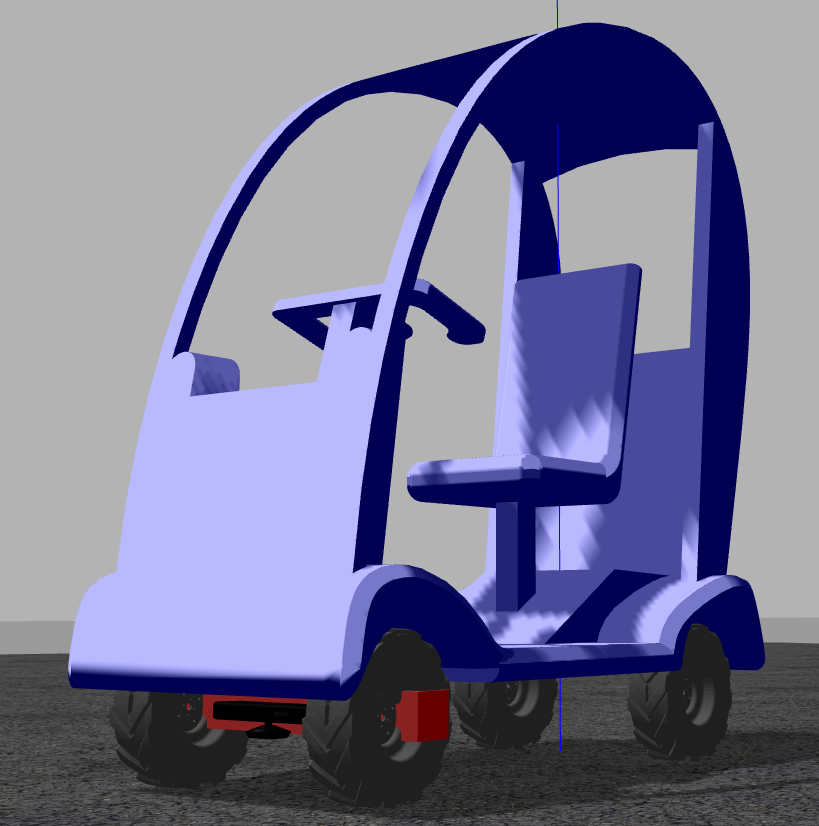
\includegraphics[width=0.75\columnwidth]{software/podcar_sim.png}
		\caption{Visual mesh simulation of vehicle with kinect sensor.}
		\label{fig:meshSim}
	\end{subfigure}
	\caption{OpenPodcar 3D simulation}
\end{figure}


A robotics simulation of the vehicle is provided for use in Gazebo 8.6.0 under ROS Kinetic and Ubuntu 16.04 (Xenial).

The physics simulation is based on a simplified vehicle geometry with two large cuboids containing the vehicles’ mass. \ref{fig:physSim} Parallel steering linkage is simulated via ODE joints forming a tracking rod. Rear drive motor and the steering linear actuator are simulated via ODE PID controllers.  Wheel geometry was measured from the physical vehicle.   Wheel forwards and lateral Coulomb friction coefficients were tuned by trial and error to produce realistic motion and steering.  The model is represented in SDF format, which is easy portable for use in other simulation and CAD systems.

There are some key differences when it comes to actuating the tracking rod between simulation and real life. On the physical robot, a linear actuator is mounted on the underside of the vehicle and attached to the front axle, which can extend/retract to angle the wheels. However, in simulation, the pivot joints that join the front wheels and the tracking rod can have a force applied directly to them without the need for a complicated actuator. This reduces the complexity of the model without affecting its behaviour, and is still appropriately accurate to real life.

There are also some similarities, for example both steering solutions implement a PID
(Proportional, Integral, Derivative) controller, that uses a proportional gain, integral function
and differential function to determine exactly how much force to apply at any given time in
order to keep the wheels at the desired angle. The parameters for the existing robot’s PID
controller have not been published, however trial and error found a proportional gain of 2,
differential weight of 1 and integral weight of 0 were adequate.

The simulation implements the same ROS interface as the physical vehicle system to enable plug and plug interoperability between them.  In the simulation, vehicle control messages are received, and vehicle sensor messages are sent by, a Gazebo plugin (podcarGazeboROSPlugin.cpp) which calls Gazebo’s simulation functions.  

Desired vehicle control commands, as for the physical vehicle, consist of (speed, angle) pairs, to command the speed of the rear wheels in m/s (speedcmd\_meterssec message) and the steering angle (wheelAngleCmd message) of the front wheels in radians.  The plugin and Gazebo implement these commands using simulated rotary and linear PID controllers and actuators, to rotate the rear wheels and linearly actuate the tracking rod respectively.

The plugin then publishes sensor messages corresponding to those from the physical vehicle. These include:  /odometry/groundTruth, a (noiseless) standard odometry format estimate for the vehicle’s pose; and /camera/image\_raw and /camera\_depth, the depth camera data.

A detailed graphical mesh model of the vehicle is provided for display, rather than physical simulation, purposes \ref{fig:meshSim}. This may be important for experiments such as virtual reality interactions between the simulated vehicle and human subjects, e.g. \cite{camara2021evaluating}, as their psychological responses may depend on the apparent size and share of the vehicle.

A basic 3D world containing the podcar and various test objects from Gazebo libraries is provided by default as shown in Fig. \ref{fig:sim_world}.

Fig. \ref{fig:sim_nodes} shows the complete ROS node configuration used during simulation, under manual joystick control.  
\begin{figure}[h]
	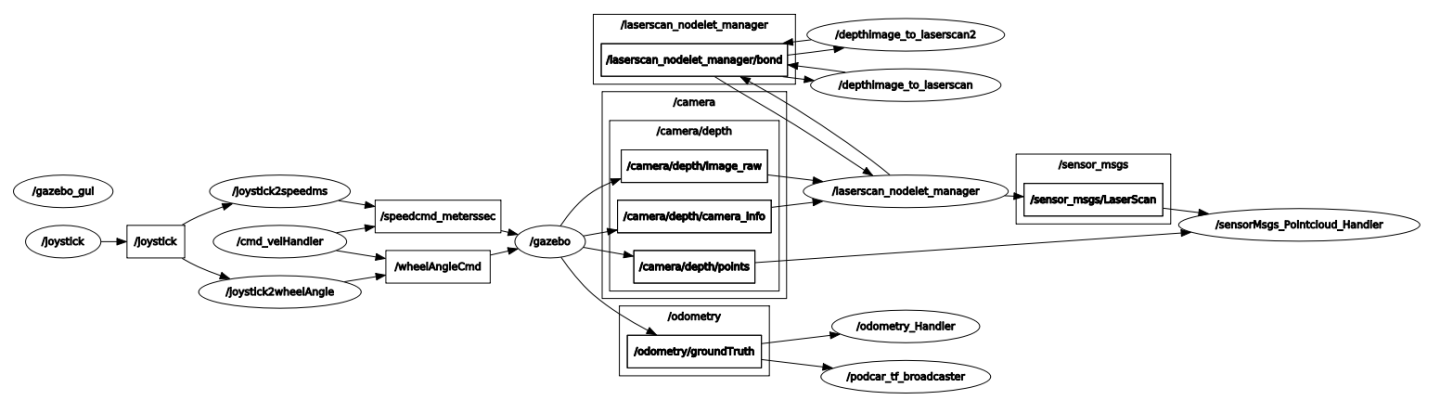
\includegraphics[width=\columnwidth]{figs_sim/sim_nodes.png}
	\caption{ROS nodes used in simulation under manual joystick control.}
	\label{fig:sim_nodes}
\end{figure}

\begin{figure}[h]
	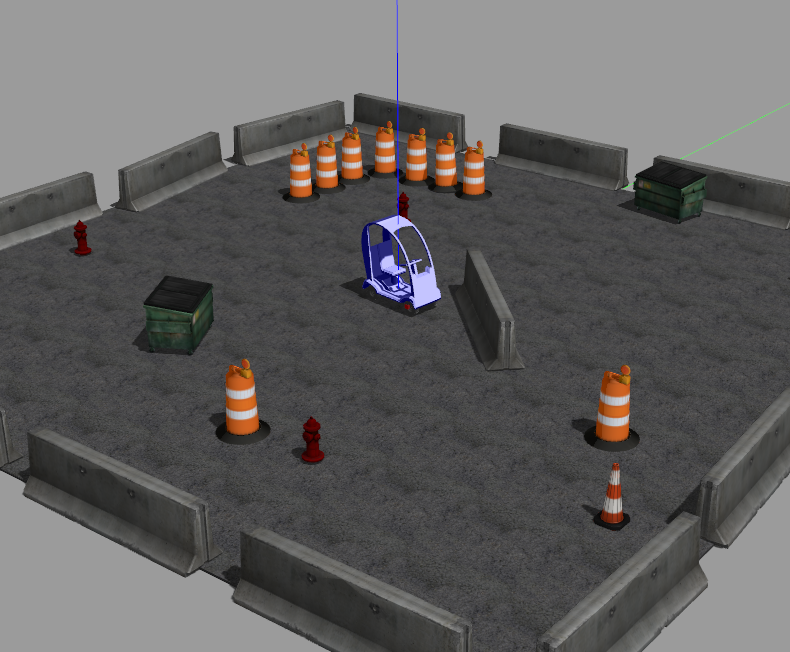
\includegraphics[width=0.5\columnwidth]{figs_sim/podcar_loaded_gazebo.png}
	\caption{Initial Gazebo simulation world}
	\label{fig:sim_world}
\end{figure}

The open source Blender 3D add-on called MapsModelsImporter [CITE] was used to create further 3D worlds representative of the University of Lincoln campus, the testing area for the podcar, and the University of Leeds campus. Before using MapsModelsImporter, RenderDoc [CITE], a free graphics debugger, must be used to capture 3D data from Google Streetviews.  


\begin{figure}
	\centering
	\begin{subfigure}{0.45\textwidth}
		\centering
		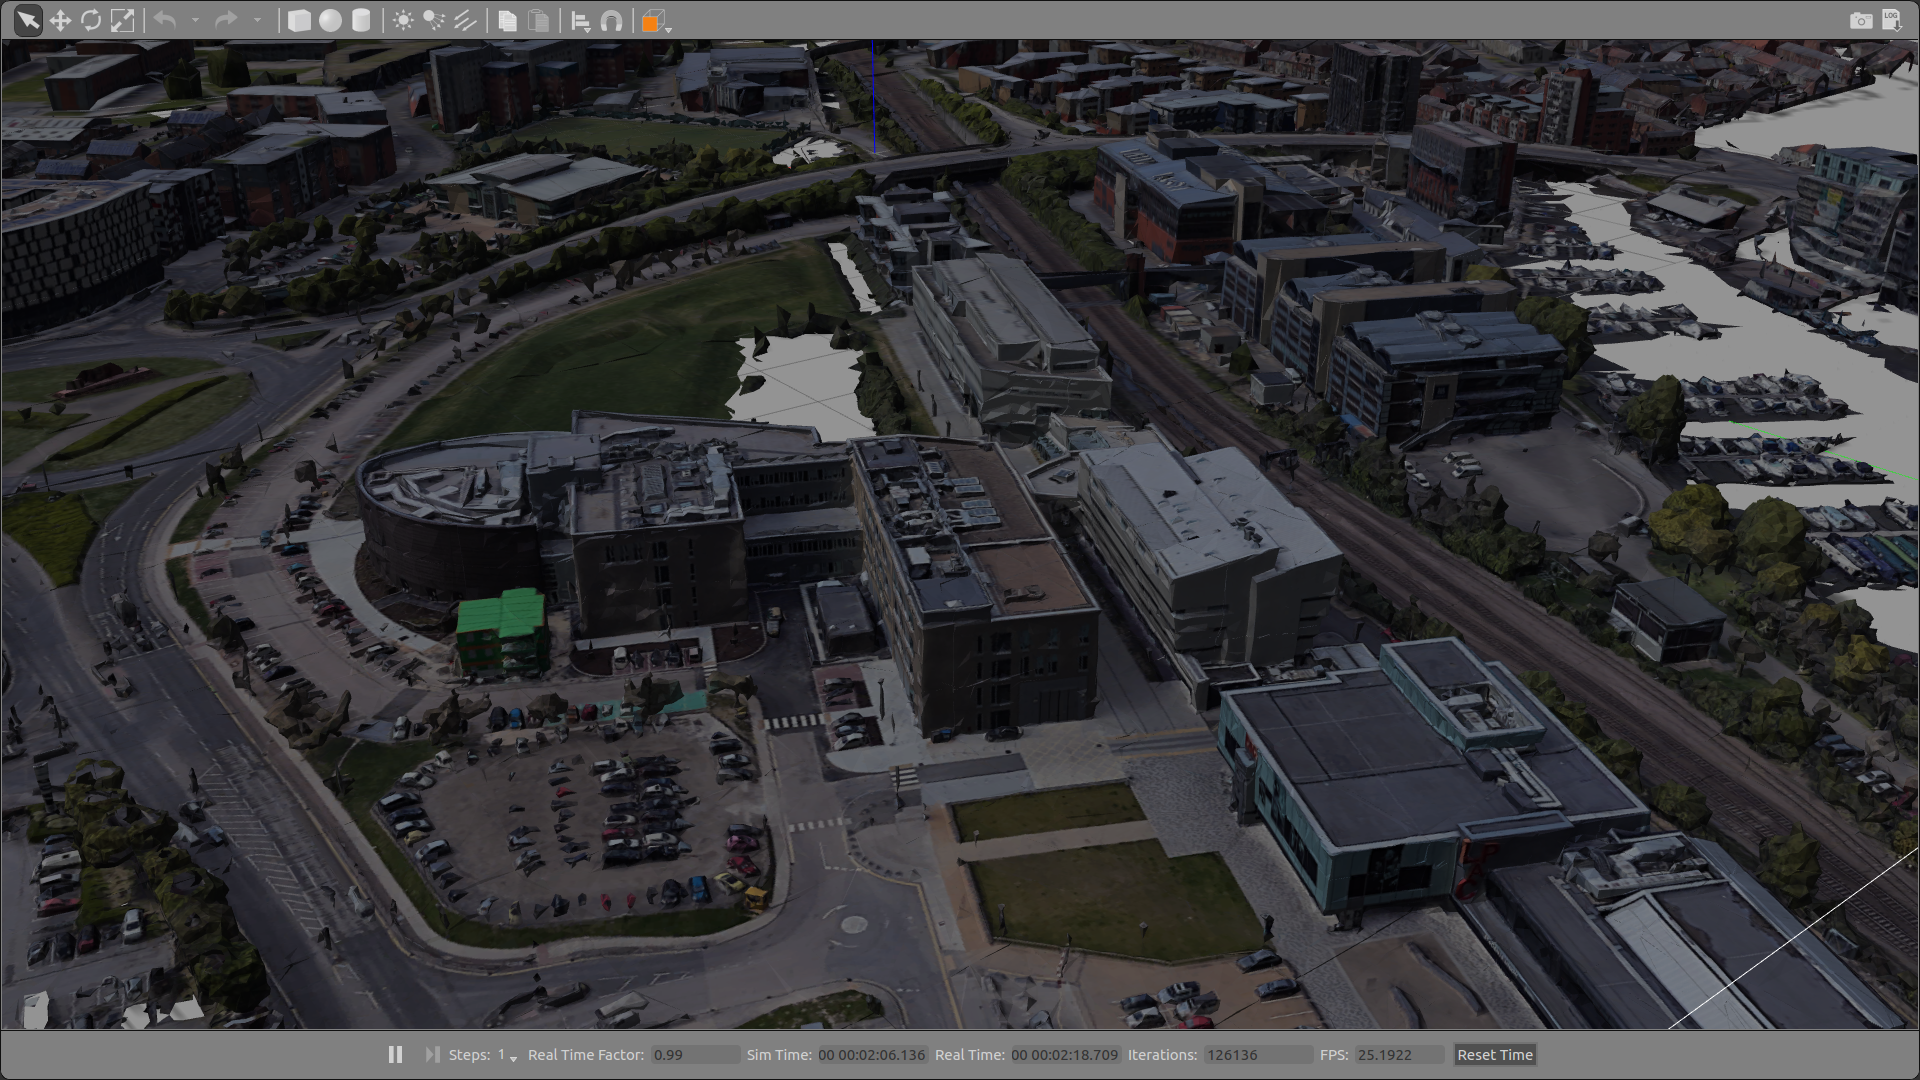
\includegraphics[width=\columnwidth]{figs_sim/INBLincoln_2.png}
		\caption{University of Lincoln's 3D world}
		\label{fig:INB_world}
	\end{subfigure}	
	\quad
	\begin{subfigure}{0.45\textwidth}
		\centering
		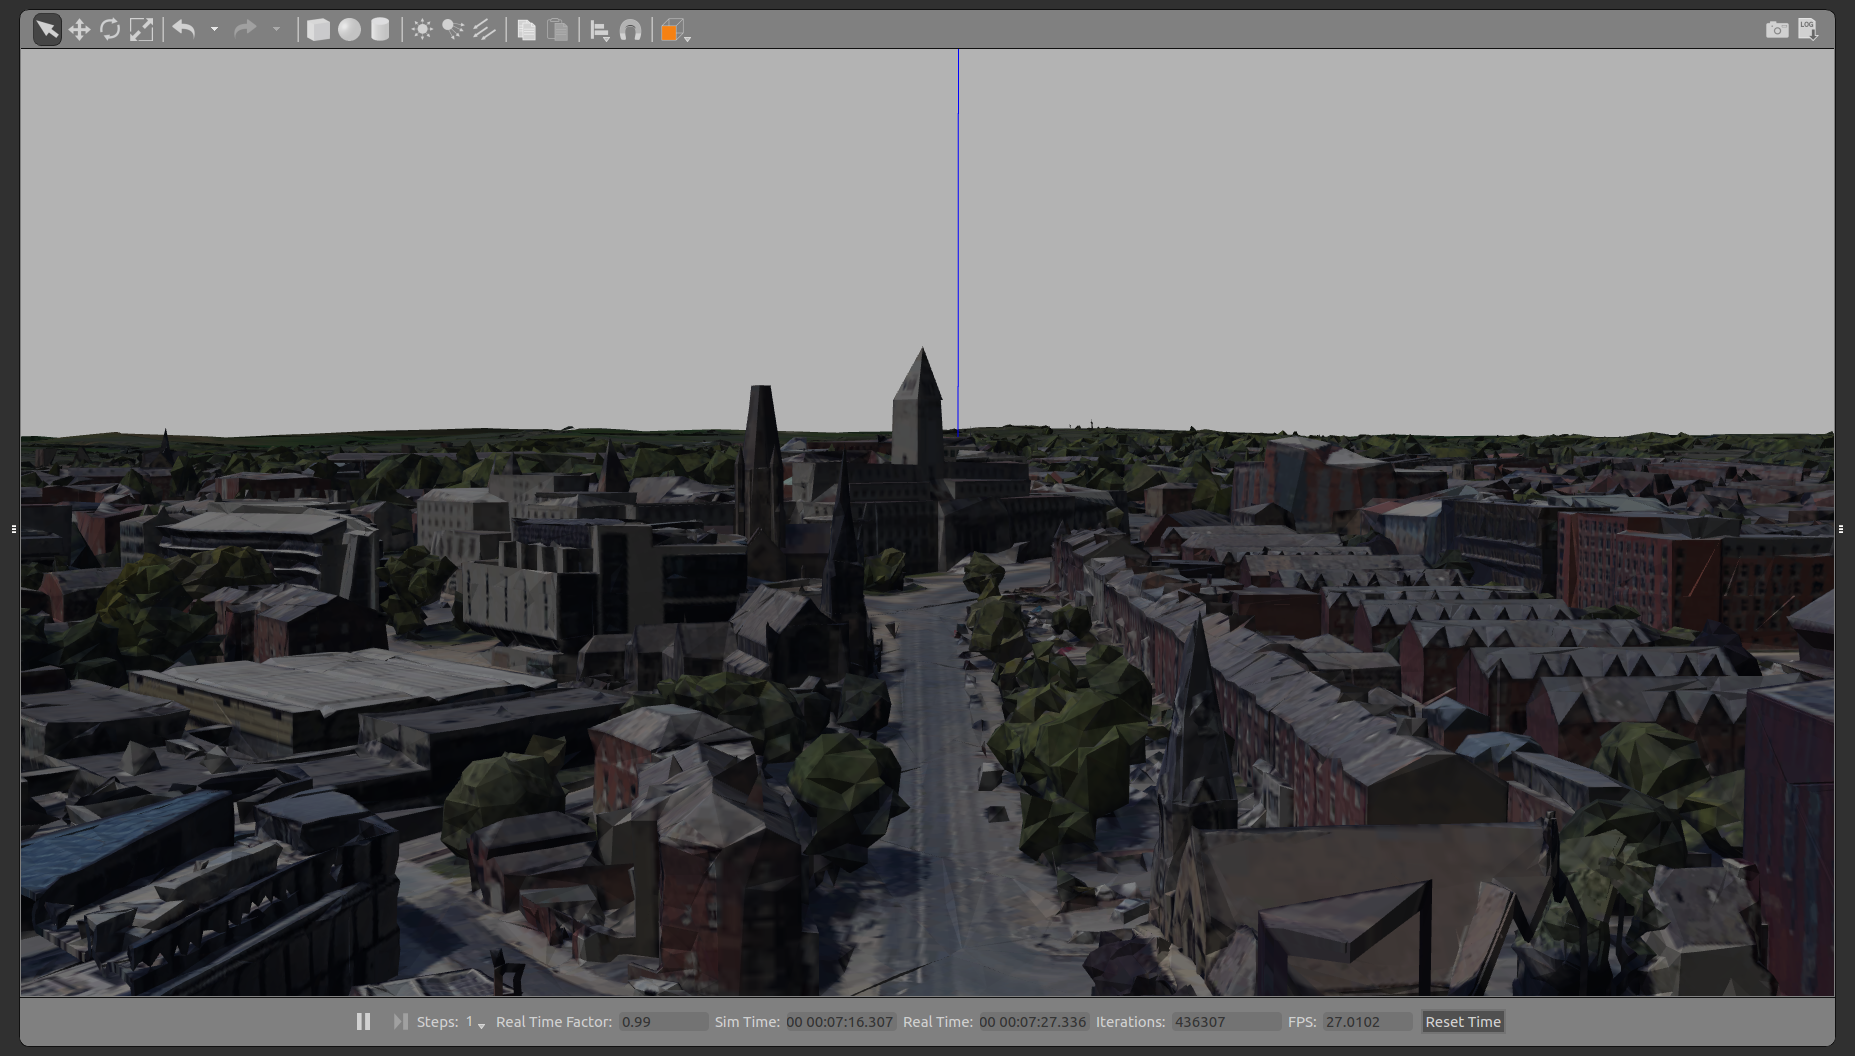
\includegraphics[width=\columnwidth]{figs_sim/woodhouseLeeds_5.png}
		\caption{University of Leeds' 3D world}
		\label{fig:Leeds_world}
	\end{subfigure}	
	\caption{OpenPodcar additional Gazebo 3D simulation worlds}
	\label{fig:gazebo_new_worlds}
\end{figure}


\subsubsection{Path planning and control (move\_base)}

Path planning is the selection of an entire desired trajectory for a robot to get from a current pose to a desired pose, where a pose is a position together with a heading direction. Path planning may be split into high level and local planning, where high level makes large scale decisions such as which way to go around obstacles, while local planning refines these choices into specific curves with optimal properties. Path control (or path following) is then the real-time process of executing a path plan by interactively monitoring the robot’s state, sending commands to motors, and trying to make the actualized path as close to the desired path as possible.  

Move\_base (wiki.ros.org/move\_base) is a ROS community standard which defines a set of message formats and a framework of ROS nodes for path planning and control. This framework allows different algorithms to plug in to it. Timed Elastic Band (TEB) \cite{rosmann2013efficient} is a local planner algorithm which has been integrated as a movebase plugin (wiki.ros.org/teb\_local\_planner).

Planning and control for car-like vehicles with a steering column is more complex than for differential drive (skid steer) vehicles which turn by having the wheels on one side rotate faster than the other. This is because differential drive vehicles are holonomic, meaning that in the absence of obstacles, they can move greedily from any pose to any other, while steered vehicles and non-holonomic, meaning that greedy motion is not guaranteed to reach a target pose and longer-term plans must be considered. The shortest possible path for a forward-driving steered vehicle is the Dubins path \cite{dubins1957curves}, which always consists of two circle arcs connected by a straight line, which is generalized to the Reeds-Shepp path when reversing is also allowed \cite{reeds1990optimal}. Parallel parking is a classic difficult path planning task for Reeds-Shepp vehicles.

Front-wheel-steering means that the front two wheels are used to steer the vehicle, with the rear wheels trailing and-or powering the vehicle. Ackermann steering is a special case of front-wheel-steering, in which the front wheels are connected to a tracking rod via two shorter steering arms arranged so that the two steering arms form a triangle with the center point of the vehicle’s rear axle when the wheels are facing forwards.  This results (TODO cite proof) in the front wheels forming the correct angles (which are different from each other) needed for the vehicle to drive in circular segments, with the circle radius determined by the steering angle. Vehicles whose possible driving motions are of this form are called Dubins Cars if they can drive only forwards, or Reeds-Shepp cars if they can drive forwards and reverse. Dubins and Reeds-Shepp cars have possible driving trajectories from pose A to pose B which consist of at most one circle arc segment and two straight lines to and from it. The donor podcar is a Reeds-Shepp car with Ackermann steering.


\begin{figure}
	\centering
	\begin{subfigure}{0.45\textwidth}
		\centering
		\includegraphics[width=0.4\columnwidth]{hardware/ackermann1.png}
		\caption{Ackermann steering}
		\label{fig:ackermann1}
	\end{subfigure}	
	\quad
	\begin{subfigure}{0.45\textwidth}
		\centering
		\includegraphics[width=0.75\columnwidth]{hardware/ackermann2.png}
		\caption{Ackermann steering}
		\label{fig:ackermann2}
	\end{subfigure}
	\caption{Ackermann steering (Source: Wikipedia; Ackermann Steering; Creative Commons.}
\end{figure}


The values for parameters such as minimum turning radius were calculated from the technical specifications of the base vehicle \cite{shopriderflagship}.

Move\_base is a set of ROS nodes that are standard for controlling robots via ROS. It enforces
conventions for being able to send messages to controllers, for example the use of Twist
messages. These messages are made up of 6 floats, the first 3 representing linear velocity in
each axis (x, y and z; forward, left and up) with the latter 3 representing angular velocity in
the same space. Move\_base requires the robot to move with these given velocities when a
Twist message is published to the /cmd vel topic (Marder-Eppstein, 2018). These standards
ensure compatibility between packages, making the addition of existing packages to a project
much easier.

Twist messages, however, don’t apply to all robots. For example, the vast majority of robots
aren’t able to move directly up in the world, so the linear z component of the message is
ignored. 
%A similar problem arises when considering ‘car-like’ steering, as they are unable to inflict an angular velocity. In this case, the angular z component is instead taken to refer to the desired angle of the steerable wheels, which resolves the incompatibility problem provided all nodes involved are aware of the difference. Alternatively, an intermediary node could be introduced that calculates the wheel angle needed to make the robot turn at a given rate, however this would be unnecessarily complex and wouldn’t have the desired effect if the robot’s linear velocity was 0.

\subsubsection{Localisation and mapping system}

Simultaneous Localisation and Mapping (SLAM) \cite{thrun2002probabilistic} is the robotic task of inferring the robot’s location at the same time as building a map of its environment, which is a classic `chicken and egg’ problem as the two subtasks depend on one another. Solving SLAM is an NP-hard problem but many standard approximations exist. Gmapping \cite{yuen2017improved} is a ROS implementation of a Rao-Blackwellized Particle Filter (RBPF)for 2D SLAM, in which “each particle carries an individual map of the environment”  The information carried by each particle overlaps, and an estimation of a map can be built based on these relationships. As the robot moves around the environment, these estimations are stored, and when a ‘feedback loop’ is closed, the estimations cascade into a portion of the completed map. These maps take the form of 2-D occupancy grids, and can be used later by the navigation stack to plan paths around the environment.

We tested GMapping for both real-time SLAM and also offline mapping. To provide reliable odometry data, we used ROS laser\_scan\_matcher package, which can serve as a stand-alone odometry estimator that matches consecutive laser scans.

Performing SLAM in 3D is more computationally challenging, but has recently become possible due to hardware acceleration provided by parallel GPU computers. We may test as part of future work some of these algorithms such as OrbSLAM based on visual features or NDT SLAM \cite{einhorn2015generic}. 

%OrbSLAM is a ROS 3D SLAM based on the Octomap algorithm, which can operate with mono visual features, or lidar or stereo camera point clouds. It maintains a voxel based map of the environment (similar to maps in the game Minecraft) and is a 3D analog of gmapping.

%NDT SLAM  (used in Autoware and ILIAD) is another 3D SLAM implementation and algorithm based on Normal Distribution Transforms \cite{einhorn2015generic}.





\subsubsection{Pedestrian Detection and Tracking}

We integrated the pedestrian detector and tracker ROS package developed as part of EU H2020 FLOBOT project. The lidar-based detections are classified by a SVM (Support Vector Machines) classifier. Then a Bayesian multi-target tracker is used to track pedestrians over time. The installation details are provided in the documentation.  


\subsection{Reuse potential and adaptability}\label{h.6wkumyl0ejrh}

%Please describe in as much detail as possible the ways in which the hardware could be reused by other researchers both within and outside of your field. This should include the use cases for the hardware, and also details of how the hardware might be modified or extended (including how contributors should contact you) if appropriate.Refer to section ``Ease of build'' where necessary.

%Please provide your thoughts on the adaptability of the hardware design. What tools and procedures would it require for other users to modify your design without your help in order to adapt them for foreseeable or even unforeseeable use.

%Also you must include details of what support mechanisms there are in place for this hardware and software (even if there is no support or support community).


\section{(4) Build Details}\label{h.l8i9vokvs0bj}

\subsection{Availability of materials and methods}\label{h.60suejv0jlzi}

%Summarise what materials have been used to construct the hardware and what methods to process the materials as well as the assembly. Provide more details or references where important materials or methods are non-standard, not globally available or produced only by one manufacturer.


\subsection{Ease of build}\label{h.wg823sgyb1e4}

%Have any measures been taken in the design to make the hardware easy to build for other users e.g. reduction of parts, features in the design to make the hardware assembly more reliable?


\subsection{Operating software and peripherals}\label{h.uz77dixfh5i4}

%If hardware requires software, details on the operating software and programming language - Please include minimum version compatibility. Additional system requirements, e.g. memory, disk space, processor, input or output devices.

%If the hardware does not require software, detail any required supporting processes or protocols required for use.

The work mainly requires Arduino IDE, Pololu Configuration Utility Manager, Ubuntu 16.04, Robot Operating System (ROS) Kinetic, Gazebo, KiCad (PCB Design). 


\subsection{Dependencies}\label{h.vr0vnjs8z9ar}

E.g. other hardware or software projects, modular components,
libraries, frameworks, incl. minimum version compatibility.

Software required for this project include:
\begin{itemize}
	\item Robot Operating System (ROS) Kinetic Kame: 
	\item Gazebo 7: 
	\item FLOBOT EU Project for people detection and tracking:
	\item KiCad for PCB Design:
	\item Arduino IDE for speed control: 
	\item Pololu Configuration Utility Manager for linear actuator control
\end{itemize}


\subsection{Hardware documentation and files location:}\label{h.nbisrsde6sc3}

\textbf{Archive for hardware documentation, build files and software}

\textbf{Name}: GitHub

\textbf{Persistent identifier:} e.g. DOI, etc.

\textbf{Project repository:} \url{https://github.com/OpenPodcar}

\textbf{Licence:} CERN-OHL-W (weakly reciprocal)

\textbf{Date published:} dd/mm/2022


This project will also seek for OSHWA certification.


\section{(5) Discussion}\label{h.90jl7wm65t65}

\subsection{Conclusions}\label{h.h3fr33ylzsnh}

Conclusions, learned lessons from design iterations, learned lessons
from use cases, summary of results.


\subsection{Future Work}\label{h.neocsr410zj}

%Further work pursued by the authors or collaborators; known issues;
%suggestions for others to improve on the hardware design or testing,,
%given what you have learned from your design iterations.

- Depth camera option
A lower cost alternative to lidar is to use a stereo camera for point cloud sensing. In this option, a StereoLabs ZedCam is mounted similarly on the vehicle roof.

- Motor controller with OSMC

- Human-Robot Interactions


\section*{Paper author contributions}\label{h.fy8hbipy6kwe}




\section*{Acknowledgements}\label{h.gu3yyarx72d6}

	The authors would like to thank Jacob Lord for creating the vehicle graphical mesh model, Yao Chen for scoping Dubins path methods and the mechanical design, Gabriel Walton for scoping simulation tools, Yicheng Zhang for helping with the 3D printer and many other useful tools for the PCB board, Zak Burrows for the PCB enclosure and assistance during some autonomous driving tests.


\section*{Funding statement}\label{h.4u1a7tugh2om}

%If the hardware resulted from funded research please give the funder
%and grant number.

	This project has received funding from EU H2020 interACT: Designing cooperative interaction of automated vehicles with other road users in mixed traffic environments under grant agreement No 723395, and from InnovateUK C19-ADVs project grant No XXXX.


\section*{Competing interests}\label{h.q1j1rznb43fl}

	The authors declare that they have no competing interests.


%\subsection{References}\label{h.6fml9tf50r5c}

%Please enter references in the Harvard style and include a DOI where
%available, citing them in the text with author and year.

	\bibliographystyle{plain}
	\bibliography{podcar}


\section*{Copyright notice}\label{h.jm5gcqv4g8x0}

\copyright~2022 The Authors. %This is an open-access article distributed under the terms of the Creative Commons Attribution 4.0 International License (CC-BY 4.0), which permits unrestricted use, distribution, and reproduction in any medium, provided the original author and source are credited. See http://creativecommons.org/ licenses/by/4.0/.



\end{document}